\documentclass[]{beamer}
\mode<presentation>
% Time-stamp: <2016-05-11 11:24:10 (jmiller)>

% beamer stuff
% Gives us the bottom line with all the goodies
\useoutertheme{infolines}
% Just the theme to use. Should be built into bemaer. Setting the
% height gets rid of a whole lot of whitespace
\usetheme[height=7mm]{Rochester}
\usefonttheme{serif}
% Usually beamer gives you navigation hyperlinks on the bottom
% right. I turned this off. It's annoying.
\setbeamertemplate{navigation symbols}{} 
% Makes my text boxes look pretty
\setbeamertemplate{blocks}[rounded][shadow=true] 
% Makes my bullet points 3d balls
\setbeamertemplate{items}[ball]

% Josh's packages
\usepackage{multimedia}
\usepackage{tabularx}
\usepackage{booktabs}
\usepackage{subfigure}
\usepackage{graphicx}
\usepackage{amsmath}
\usepackage{latexsym}
\usepackage{mathrsfs}

% Packages for me
\usepackage{amsmath,amssymb,latexsym}
\usepackage[mathscr]{eucal}
\usepackage{mathrsfs}
\usepackage{verbatim}
\usepackage{braket}
\usepackage{listings}
\usepackage{amsthm}
\usepackage{xcolor}
%\usepackage[usenames,dvipsnames,svgnames,table]{xcolor}
\usepackage{fancybox}
\usepackage{animate}
% \usepackage{media9}
\usepackage{multicol}
\usepackage{mdframed}
%\usepackage{scalerel}
\usepackage{hyperref}

% Macros

%Blackboard Bold
\newcommand{\R}{\mathbb{R}}
\newcommand{\Z}{\mathbb{Z}}
\newcommand{\N}{\mathbb{N}}
\newcommand{\Q}{\mathbb{Q}}
\newcommand{\A}{\mathbb{A}}
\newcommand{\E}{\mathbb{E}}
% other
\newcommand{\eval}{\biggr\rvert} %evaluated at
\newcommand{\myvec}[1]{\mathbf{#1}} % vectors for me
% total derivatives 
\newcommand{\diff}[2]{\frac{d #1}{d #2}} 
\newcommand{\dd}[1]{\frac{d}{d #1}}
% partial derivatives
\newcommand{\pd}[2]{\frac{\partial #1}{\partial #2}} 
\newcommand{\pdd}[1]{\frac{\partial}{\partial #1}} 
% Order operator
\DeclareRobustCommand{\orderof}{\ensuremath{\mathcal{O}}}

% tikz
\usepackage{tikz}
\usetikzlibrary{arrows}
\usepackage{pgfplots}


% Keys to support piece-wise uncovering of elements in TikZ pictures:
% \node[visible on=<2->](foo){Foo}
% \node[visible on=<{2,4}>](bar){Bar}   % put braces around comma expressions
% 
% Internally works by setting opacity=0 when invisible, which has the 
% adavantage (compared to \node<2->(foo){Foo} that the node is always there, hence
% always consumes space plus that coordinate (foo) is always available.
% 
% The actual command that implements the invisibility can be overriden
% by altering the style invisible. For instance \tikzsset{invisible/.style={opacity=0.2}}
% would dim the "invisible" parts. Alternatively, the color might be set to white, if the
% output driver does not support transparencies (e.g., PS) 
% 
\tikzset{
  invisible/.style={opacity=0},
  visible on/.style={alt={#1{}{invisible}}},
  alt/.code args={<#1>#2#3}{%
    \alt<#1>{\pgfkeysalso{#2}}{\pgfkeysalso{#3}} % \pgfkeysalso doesn't change the path
  },
}

% define a really nice visible "purple"
\definecolor{gimppurple}{HTML}{AD26FB}
% a light grey
\definecolor{lightgrey}{HTML}{E0E0E0}
% for highlighting
\definecolor{deepblue}{rgb}{0,0,0.5}
\definecolor{deepred}{rgb}{0.6,0,0}
\definecolor{deepgreen}{rgb}{0,0.5,0}

% fonts
% Default fixed font does not support bold face
\DeclareFixedFont{\ttb}{T1}{txtt}{bx}{n}{12} % for bold
\DeclareFixedFont{\ttm}{T1}{txtt}{m}{n}{12}  % for normal

% Python style for highlighting
\newcommand\pythonstyle{\lstset{
language=Python,
basicstyle=\ttm\color{deepblue},
otherkeywords={self},
keywordstyle=\ttb\color{gimppurple},
emph={__init__},           
emphstyle=\ttb\color{deepred},
commentstyle=\ttfamily\color{deepred},
stringstyle=\color{deepgreen},
identifierstyle=\color{black},
frame=tb,                     
showstringspaces=false        
}}

% Python environment
\lstnewenvironment{python}[1][]
{
\pythonstyle
\lstset{#1}
}
{}

\newcommand{\backupbegin}{
   \newcounter{finalframe}
   \setcounter{finalframe}{\value{framenumber}}
}
\newcommand{\backupend}{
   \setcounter{framenumber}{\value{finalframe}}
}

\title[Comp. Phys.]{Solving Physics Problems on a Computer}
\author[J. Miller]{Jonah M. Miller}
\institute[PI]{\color{blue}Perimeter Institute for Theoretical Physics}

\date[Lunch \& Learn]{\color{black}Lunch and Learn\\May 5, 2016}

\begin{document}

\begin{frame}[plain]
\titlepage
\end{frame}

\begin{frame}{Agenda (time permitting)}
\tableofcontents
\end{frame}

\section{Throwing Darts for $\pi$}
\label{sec:darts}

\begin{frame}
  \frametitle{The Random Darts Player}
  \begin{columns}
    \column{6cm}
    \begin{center}
      \animategraphics[width=6cm,every=1,autoplay,loop]{1}{figures/darts-frame/darts-frame-}{0}{5}
    \end{center}
    \column{6cm}
    \begin{center}
      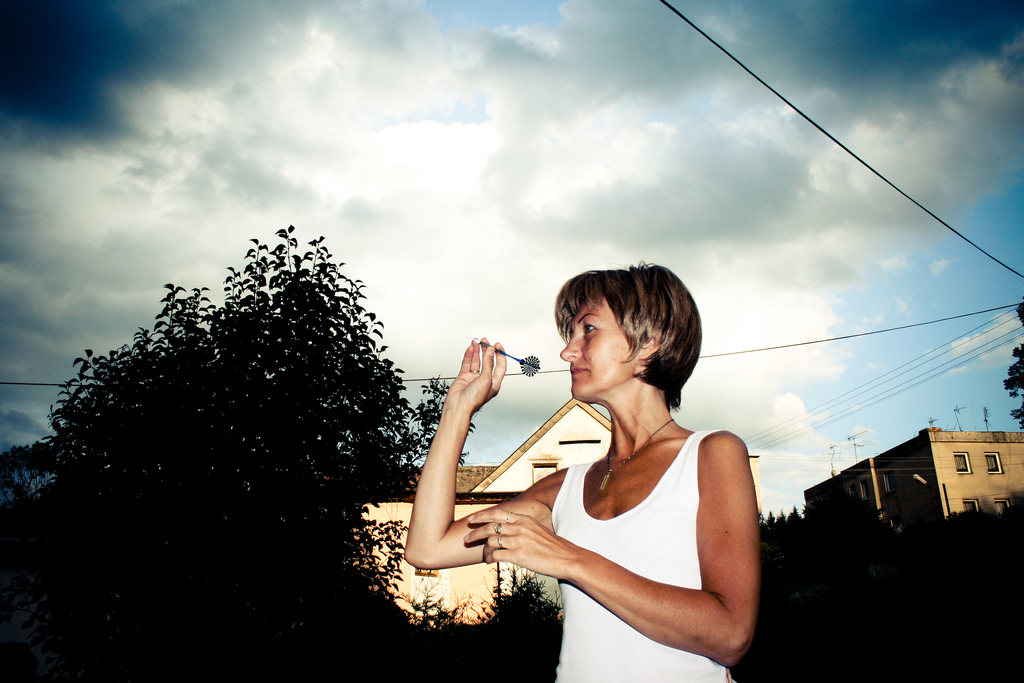
\includegraphics[width=6cm]{figures/Darts_gameplay}\\
      {\footnotesize Source: Wikimedia Commons}
    \end{center}
  \end{columns}
\end{frame}

\begin{frame}
  \frametitle{The Darts Tell us the Area of the Ring!}
  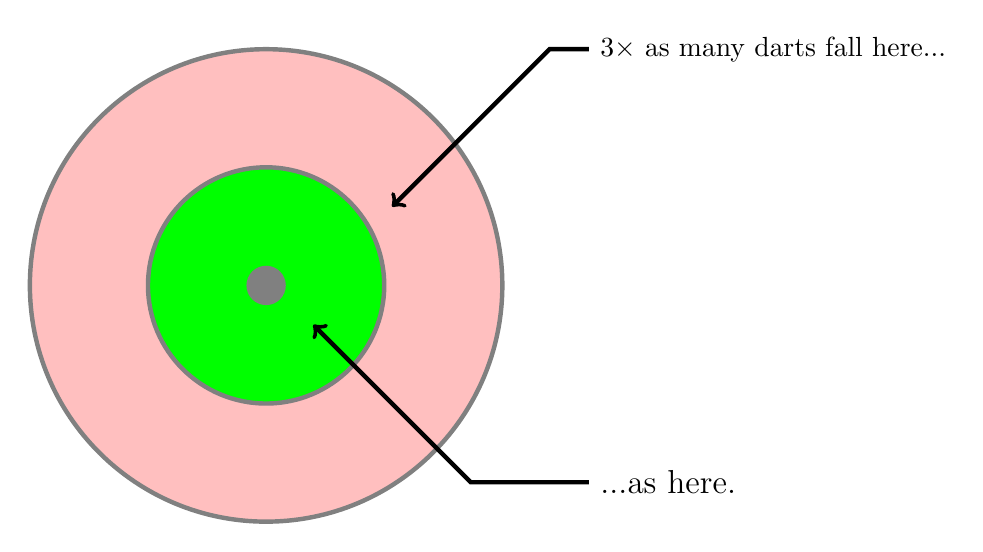
\begin{tikzpicture}
      \coordinate (bcenter) at (3.4cm,4cm);
      \fill[color=pink] (bcenter) circle(3cm);
      \fill[color=green] (bcenter) circle (1.5cm);
      \draw[color=gray,ultra thick] (bcenter) circle (1.5cm);
      \draw[color=gray,ultra thick] (bcenter) circle (3cm);
      \fill[color=gray] (bcenter) circle (0.25cm);
      \draw[color=black,ultra thick,<-] 
      (5cm,5cm) --(7cm,7cm) 
      -- (7.5cm,7cm)
      node[right] {$3\times$ as many darts fall here...};
      \draw[color=black,ultra thick,<-]
      (4cm,3.5cm) -- (6cm,1.5cm) 
      -- (7.5cm,1.5cm) 
      node[right] {\large...as here.};
    \end{tikzpicture}
\end{frame}

\begin{frame}
  \frametitle{Areas and $\pi$}
  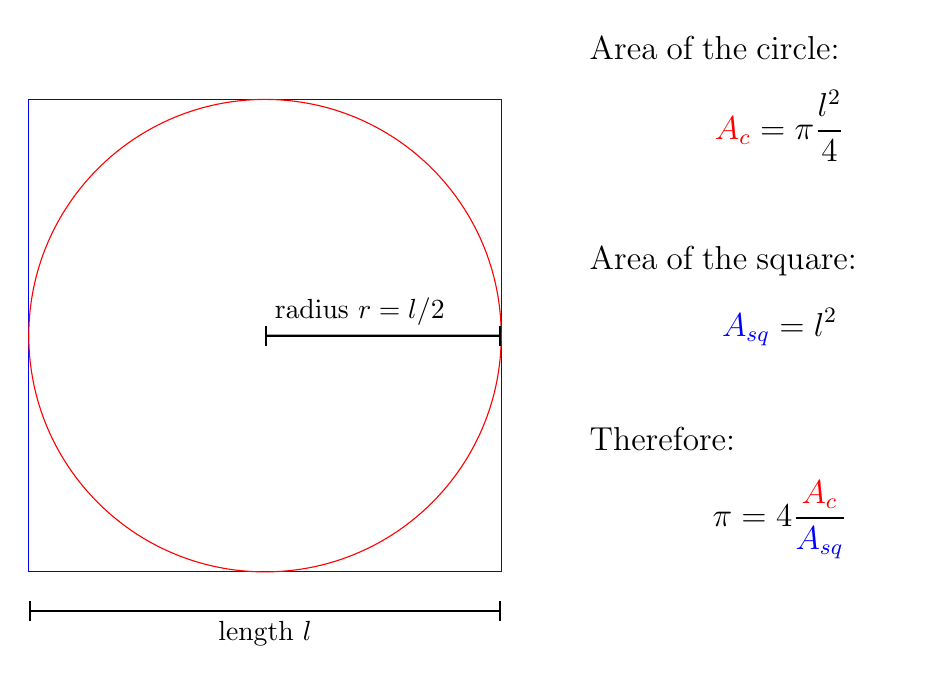
\begin{tikzpicture}
    \coordinate(bcenter) at (4cm,4cm);
    \draw[color=blue] (1,1) rectangle (7,7);
    \draw[color=red] (bcenter) circle (3cm);
    \draw[thick,|-|] (1,0.5) -- (7,0.5);
    \draw (4,0.5) node[below] {length $l$};
    \draw[thick,|-|] (bcenter) -- (7,4);
    \draw (4cm,4.3cm) node[right] {radius $r = l/2$};
    \draw (8,7) node[right,text width=4cm] 
    {\large Area of the circle:
      $$\qquad {\color{red}A_{c}} = \pi \frac{l^2}{4}$$};
    \draw (8,4.5) node[right,text width=4cm]
    {\large Area of the square:
      $$\qquad {\color{blue}A_{sq}} = l^2$$};
    \draw (8,2) node[right,text width=4cm]
    {\large Therefore:
      $$\qquad \pi = 4\frac{\color{red}A_c}{\color{blue}A_{sq}}$$};
  \end{tikzpicture}
\end{frame}

\begin{frame}[fragile]
  \frametitle{Darts and $\pi$}
  \begin{center}
    {\Large$\pi \approx 4\frac{\text{number of darts in circle}}{\text{number of darts in square}}$}
  \end{center}
\begin{python}
def throw_dart():
    x = random.uniform(rgl_min,rgl_max)
    y = random.uniform(rgl_min,rgl_max)
    return x,y
for i in range(darts_max):
    x,y = throw_dart()
    if in_circle(x,y):
        darts_in_circle += 1
    total_darts += 1
    pi = 4*(darts_in_circle/float(total_darts))
\end{python}
\end{frame}

\begin{frame}
  \frametitle{Darts and $\pi$}
  \begin{center}
    {\Large$\pi \approx 4\frac{\text{number of darts in circle}}{\text{number of darts in square}}$}
    \animategraphics[width=12cm,every=1,autoplay,loop,trim=0 4cm 0 1cm]{5}{figures/monte_carlo_for_pi/monte_carlo_for_pi-}{0}{99}
    \end{center}
\end{frame}

\begin{frame}
  \frametitle{Applications}
  \setlength{\unitlength}{1cm}
  \begin{picture}(12,8)
    \put(6,4.5){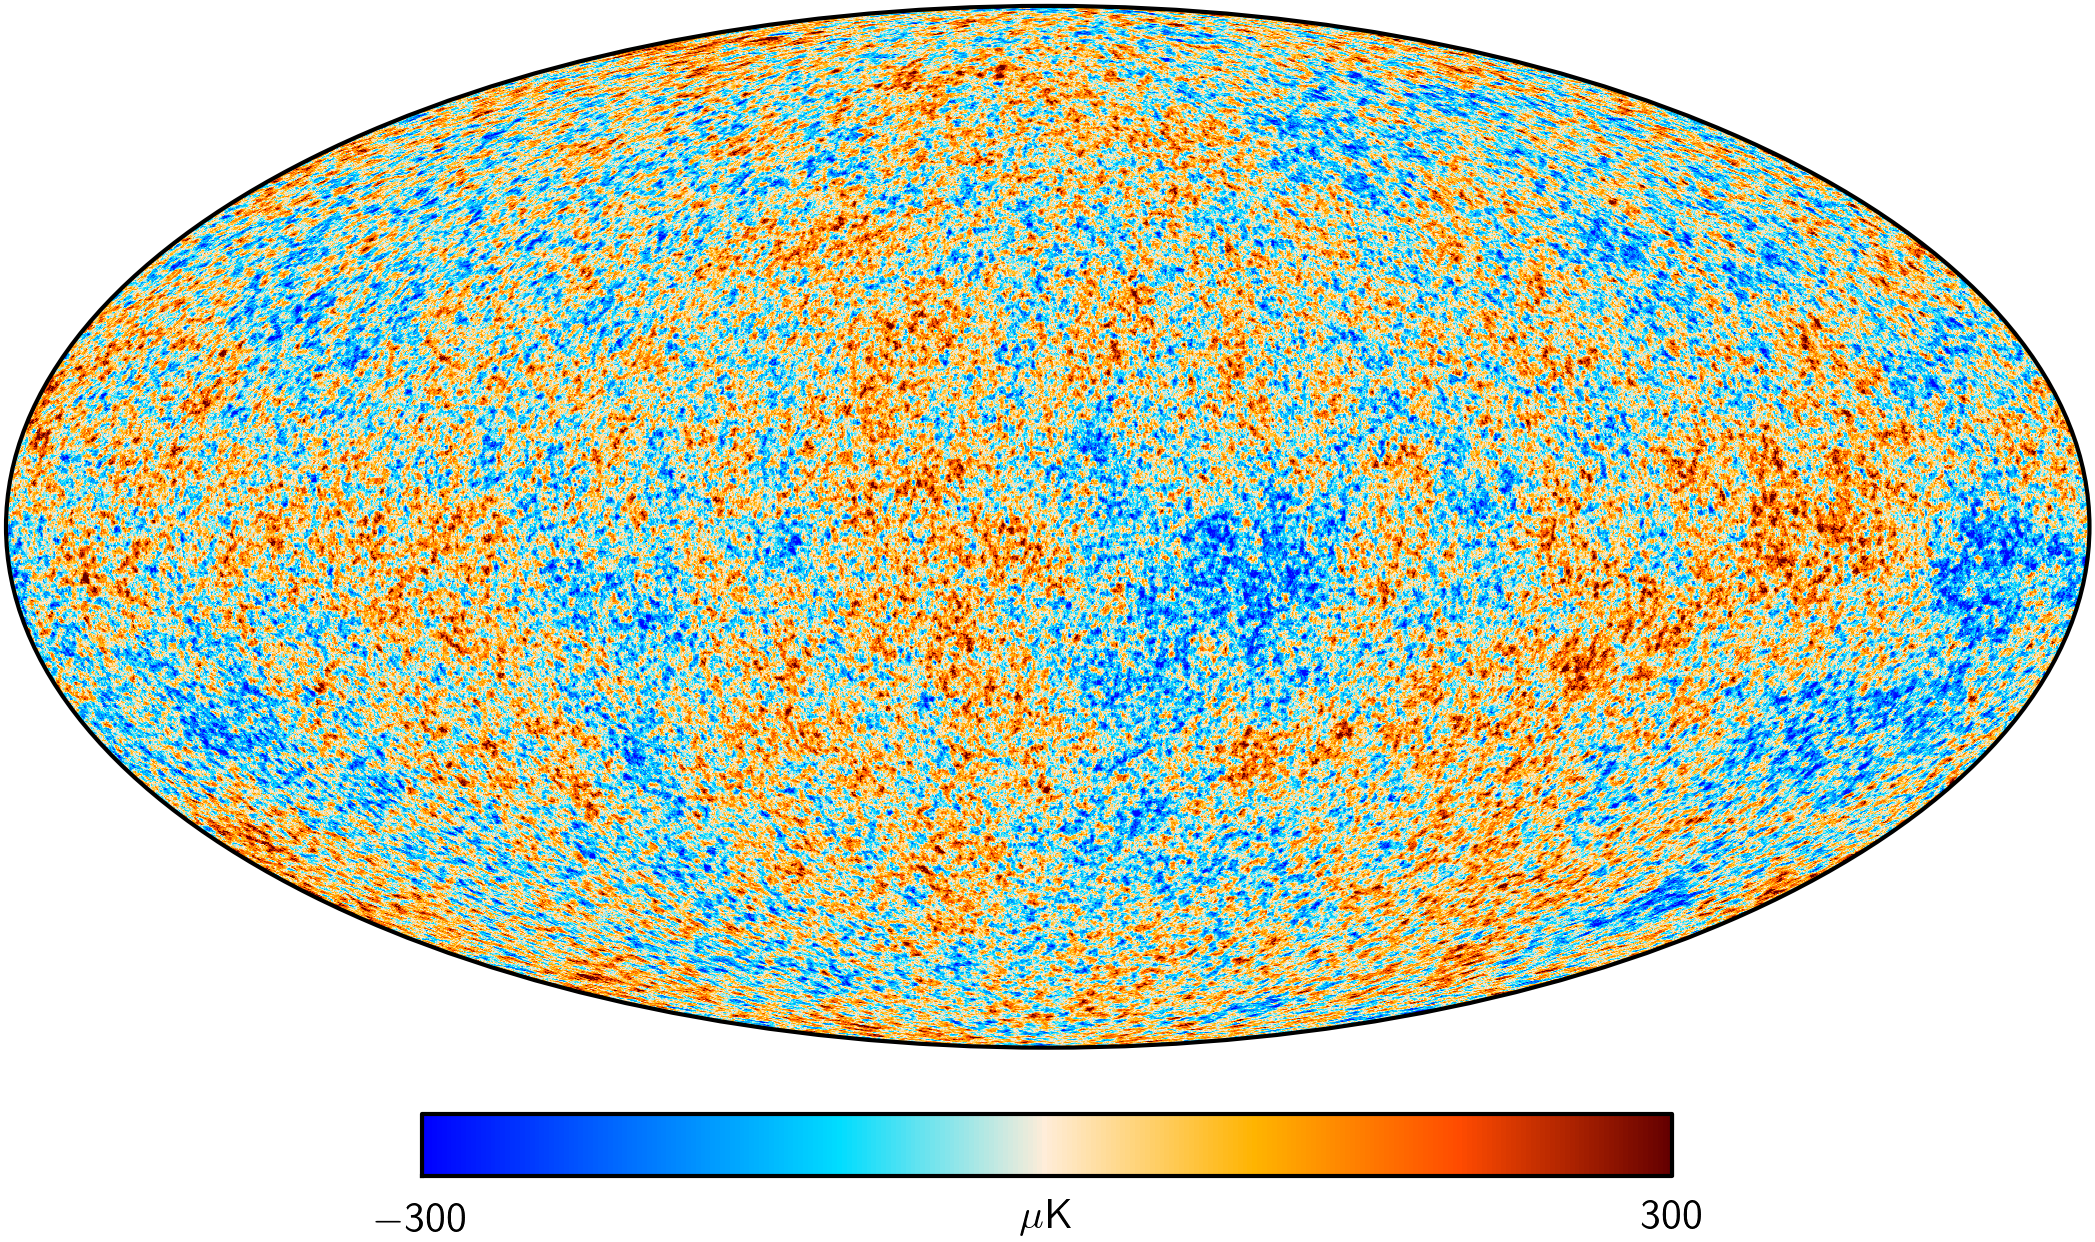
\includegraphics[width=6cm]{figures/2015_SMICA_CMB}}
    \put(6.75,4.2){\footnotesize Source: Planck Collaboration}
    \put(0,0){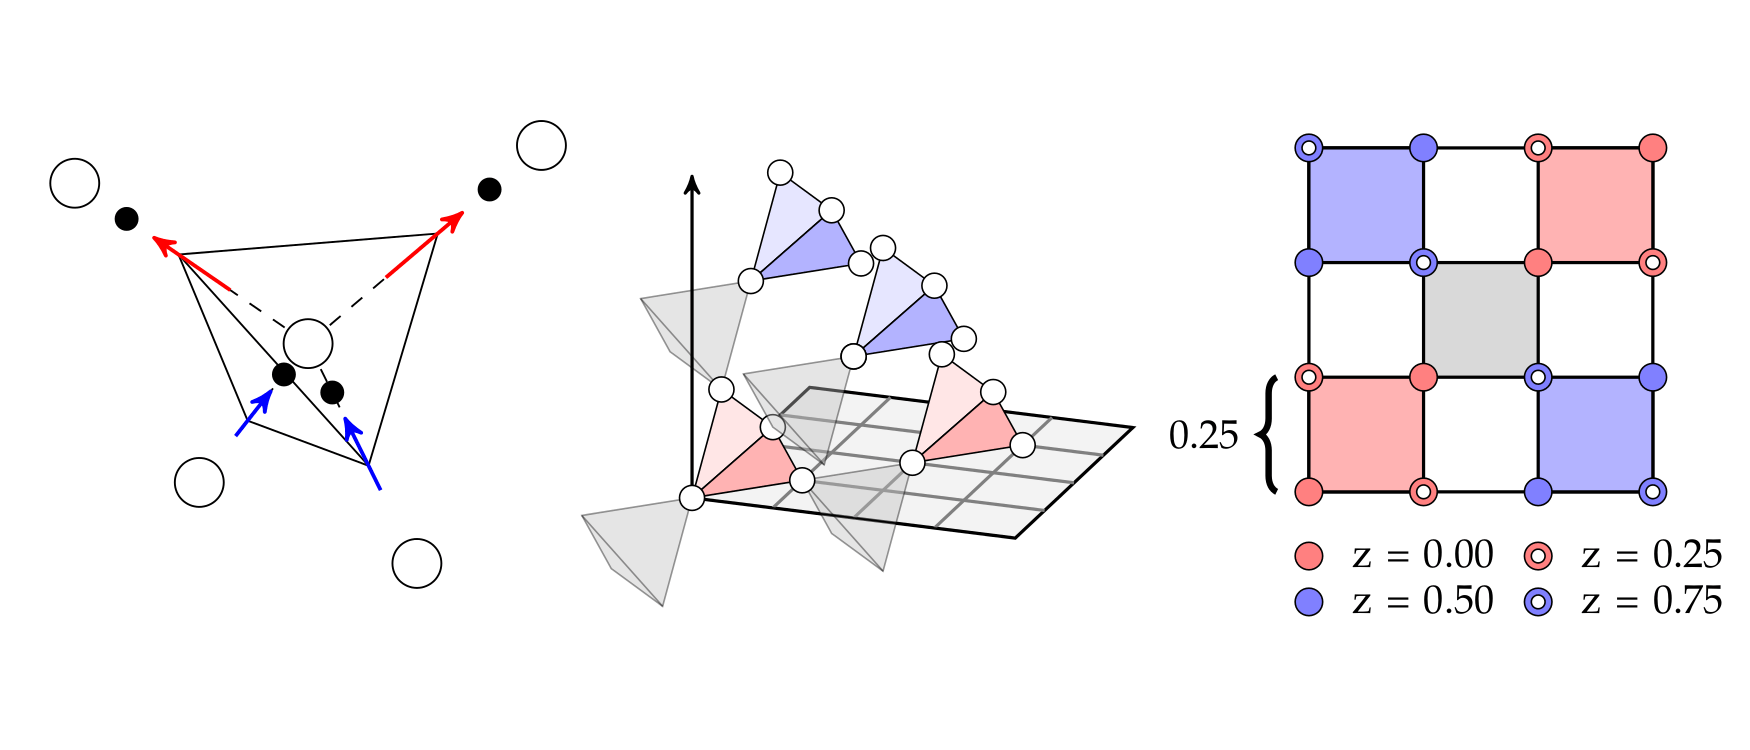
\includegraphics[height=4cm,trim=20cm 5cm 22cm 5cm,clip]{figures/researchBanner}}
    \put(1,0){\footnotesize Source: Brian Yee}
    \put(6.5,0){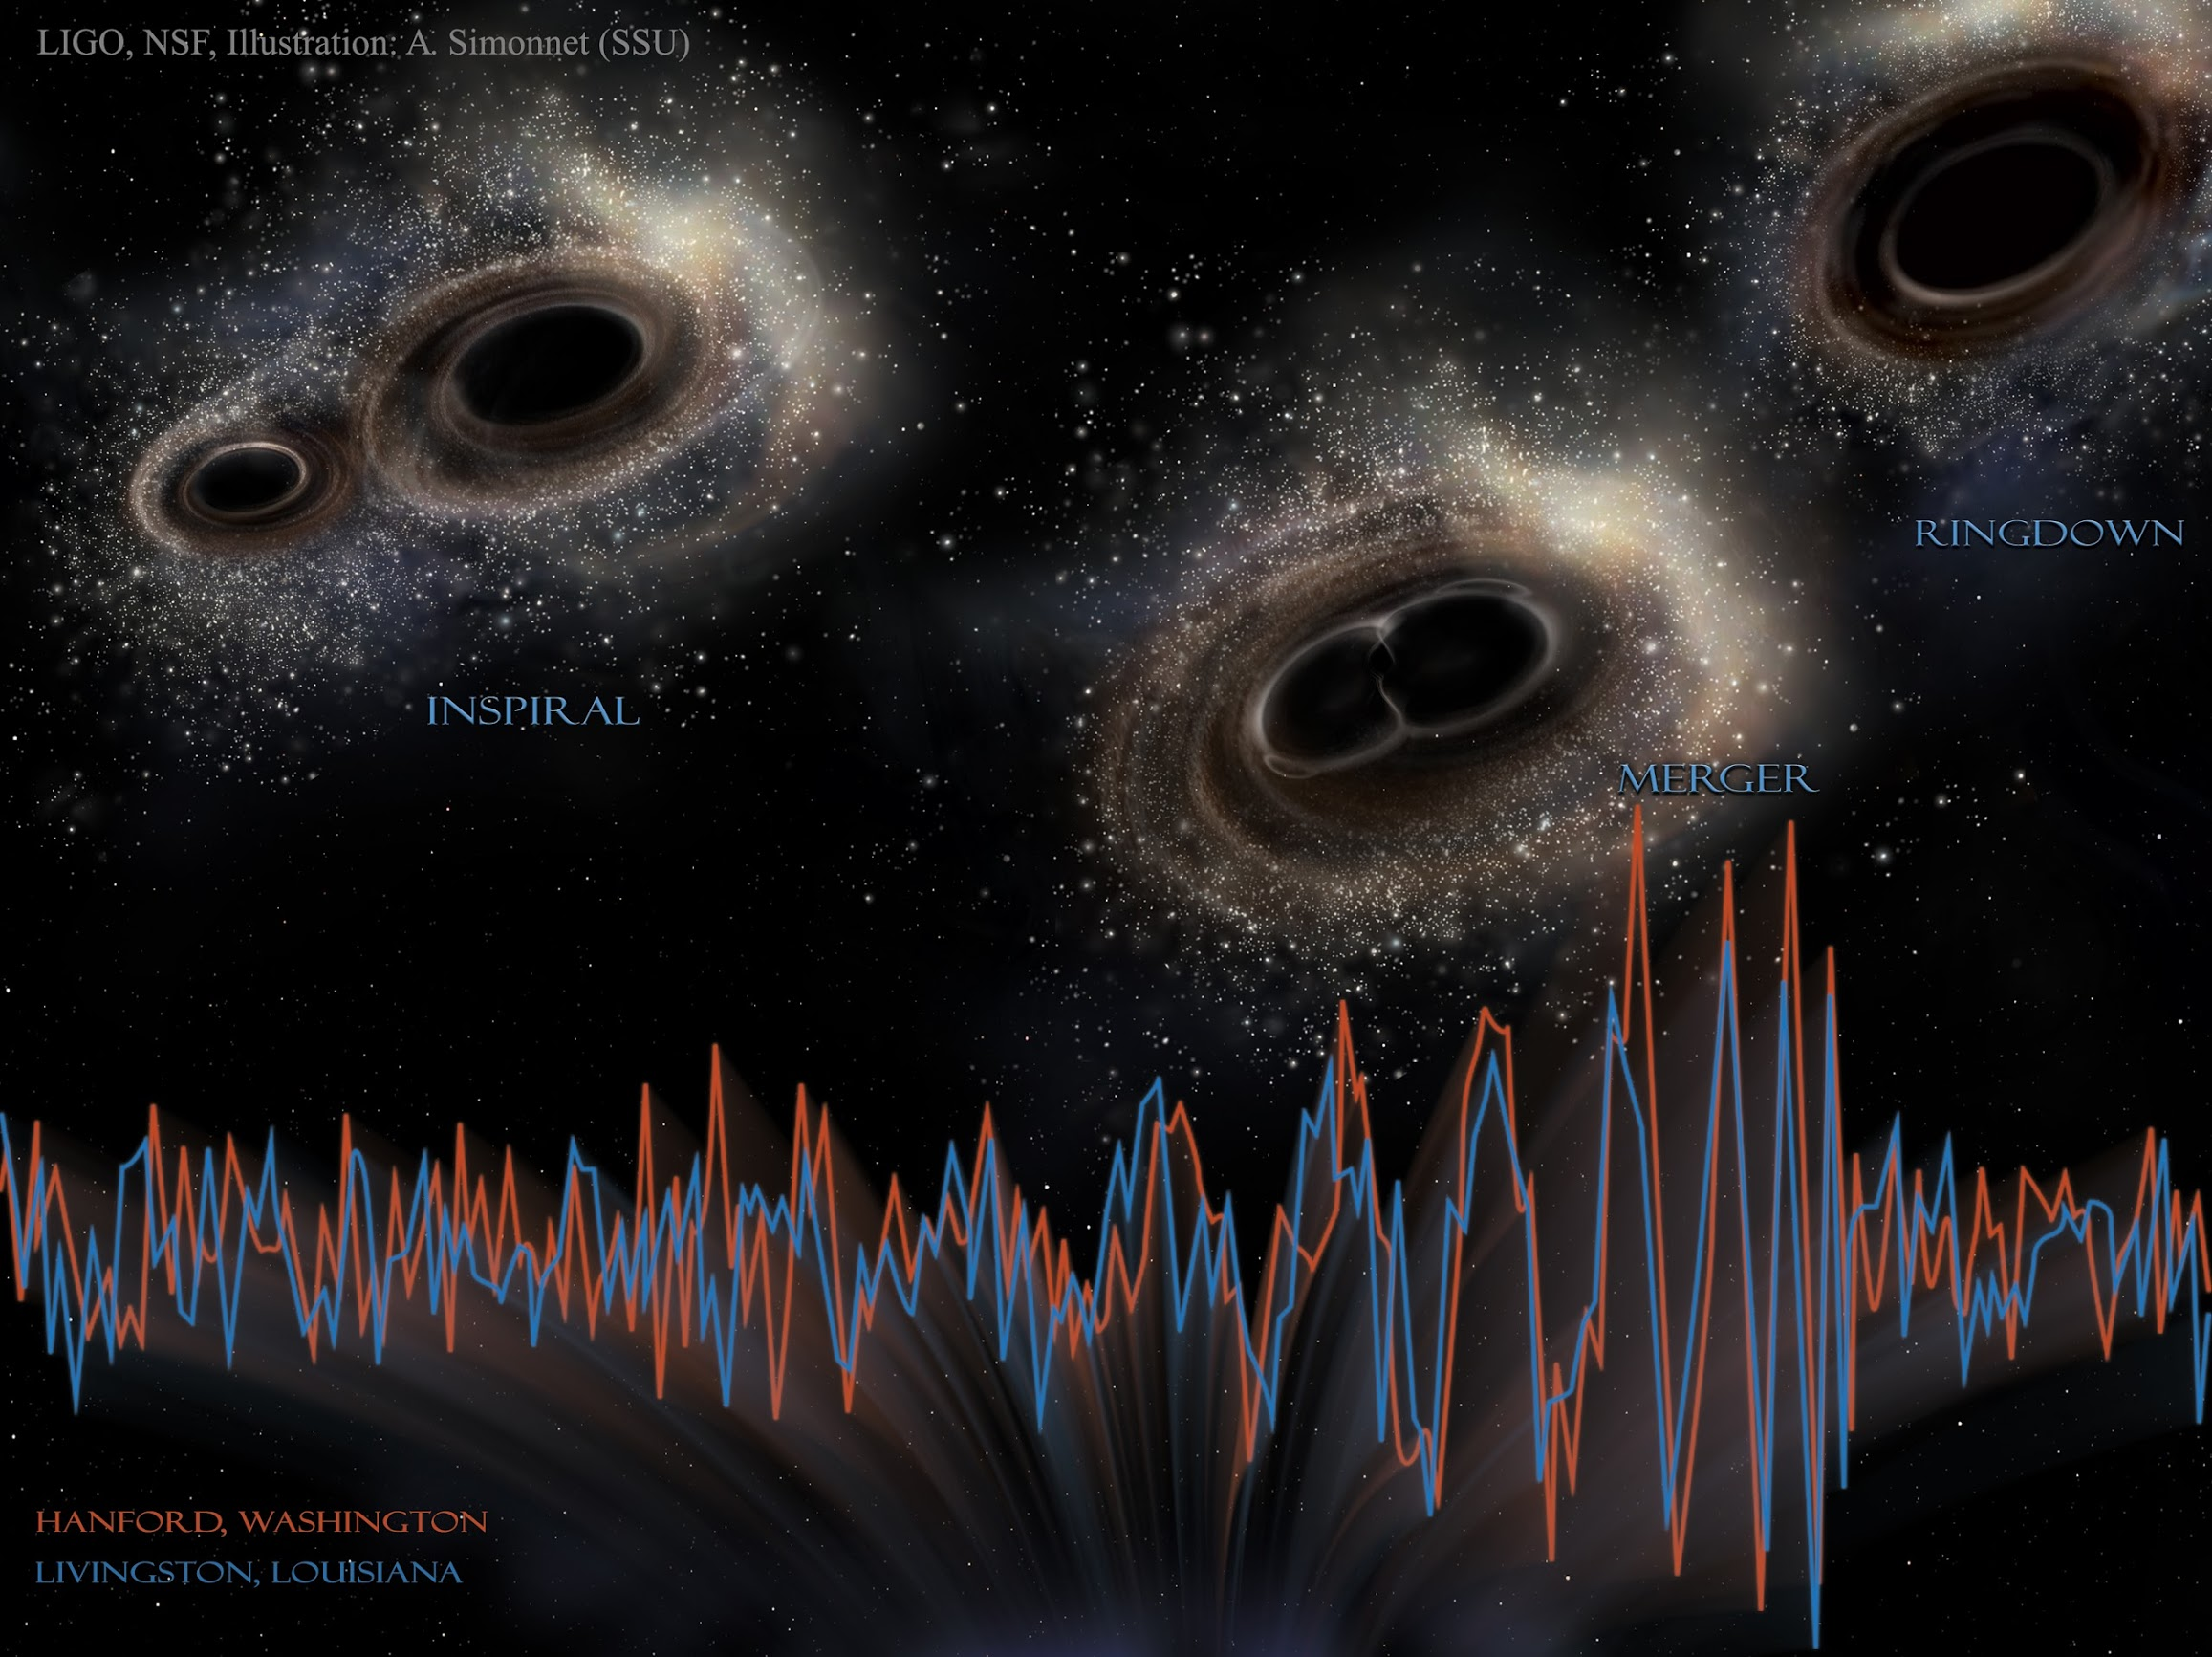
\includegraphics[height=3.7cm]{figures/BHmerger_LIGO_3600}}
    \put(0,4){\animategraphics[height=4cm,autoplay,loop]{8}{figures/no-boundary-de-sitter-monte-carlo-3d/frame_}{0}{49}}   
  \end{picture}
\end{frame}

\section{Planetary Orbits a la Newton}
\label{sec:newton}

\begin{frame}
  \frametitle{Newton's Laws}
  \resizebox{12cm}{!}{
    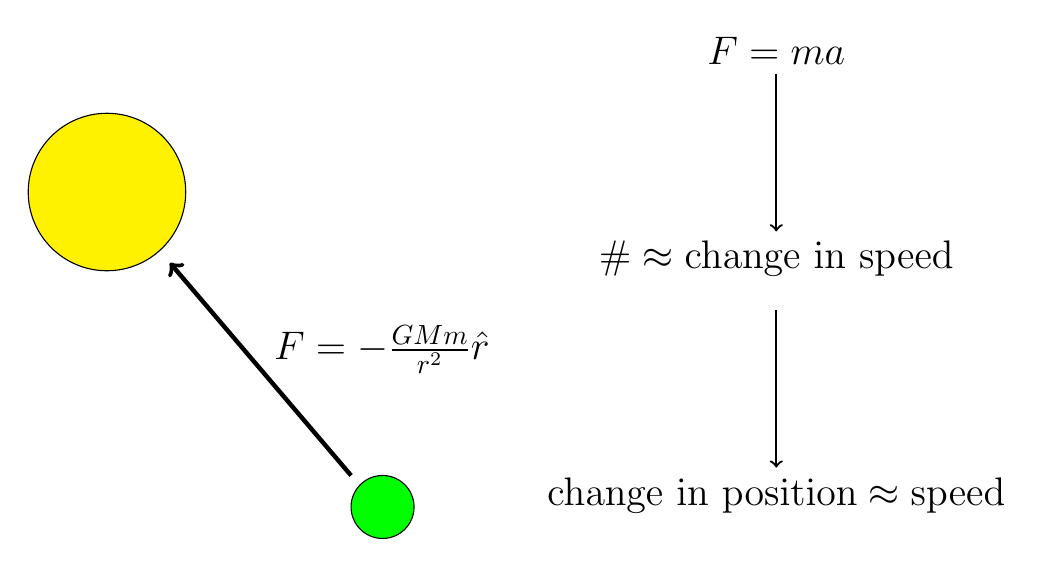
\begin{tikzpicture}
    \filldraw[draw=black,fill=yellow] (1.5,6) circle (1cm);
    \filldraw[draw=black,fill=green] (5,2) circle(0.4cm);
    \draw[ultra thick,black,->] (4.6,2.4) -- (2.3,5.1);
    \draw (3.5,4) node[right]{\Large $F = -\frac{G M m}{r^2}\hat{r}$};
    \draw (10,7.5) node[above]{\Large $F = m a$};
    \draw[thick,black,->] (10,7.5) -- (10,5.5);
    \draw (10,5.5) node[below]{\Large $\# \approx \text{change in speed}$};
    \draw (10,2.5) node[below]{\Large $\text{change in position} \approx \text{speed}$};
    \draw[thick,black,->] (10,4.5) -- (10,2.5);
  \end{tikzpicture}
}
\end{frame}

\begin{frame}
  \frametitle{Predict the Future Given Information Now}
  \begin{Large}
  \begin{center}
    \begin{tabular}{c | c}
      What we have now & What we get in the future \\
      \hline
      position $(x,y)$ & velocity $(v_x,v_y)$ \\ 
      [1ex]
      velocity $(v_x,v_y)$ & position $(x,y)$
    \end{tabular}
  \end{center}
\end{Large}
\end{frame}

\begin{frame}[fragile]
  \frametitle{The Iterative Algorithm: Forward Euler}
\begin{python}
for i in range(1,num_times):
    # update positions
    x[i] = x[i-1] + vx[i-1]*dt
    y[i] = y[i-1] + vy[i-1]*dt
    # update velocities
    ax,ay = get_acceleration(x[i-1],y[i-1])
    vx[i] = vx[i-1] + ax*dt
    vy[i] = vy[i-1] + ay*dt
\end{python}
\end{frame}

\begin{frame}
  \frametitle{Results}
  \begin{columns}
    \column{6cm}
    \begin{center}
      \animategraphics[height=4cm,every=1,autoplay,loop]{5}{figures/forward-euler-ypert-circle/frame-}{001}{085}
      \animategraphics[height=4cm,every=1,autoplay,loop]{5}{figures/forward-euler-ypert-ellipse/frame-}{001}{092}
    \end{center}
    \column{6cm}
    \begin{center}
      \animategraphics[height=4cm,every=1,autoplay,loop]{5}{figures/forward-euler-ypert-hyperbola/frame-}{001}{085}
      \animategraphics[height=4cm,every=1,autoplay,loop]{5}{figures/forward-euler-ypert-spiral/frame-}{001}{092}
    \end{center}
  \end{columns}
\end{frame}

\begin{frame}
  \frametitle{Applications}
  \begin{columns}
    \column{6cm}
     \begin{center}
       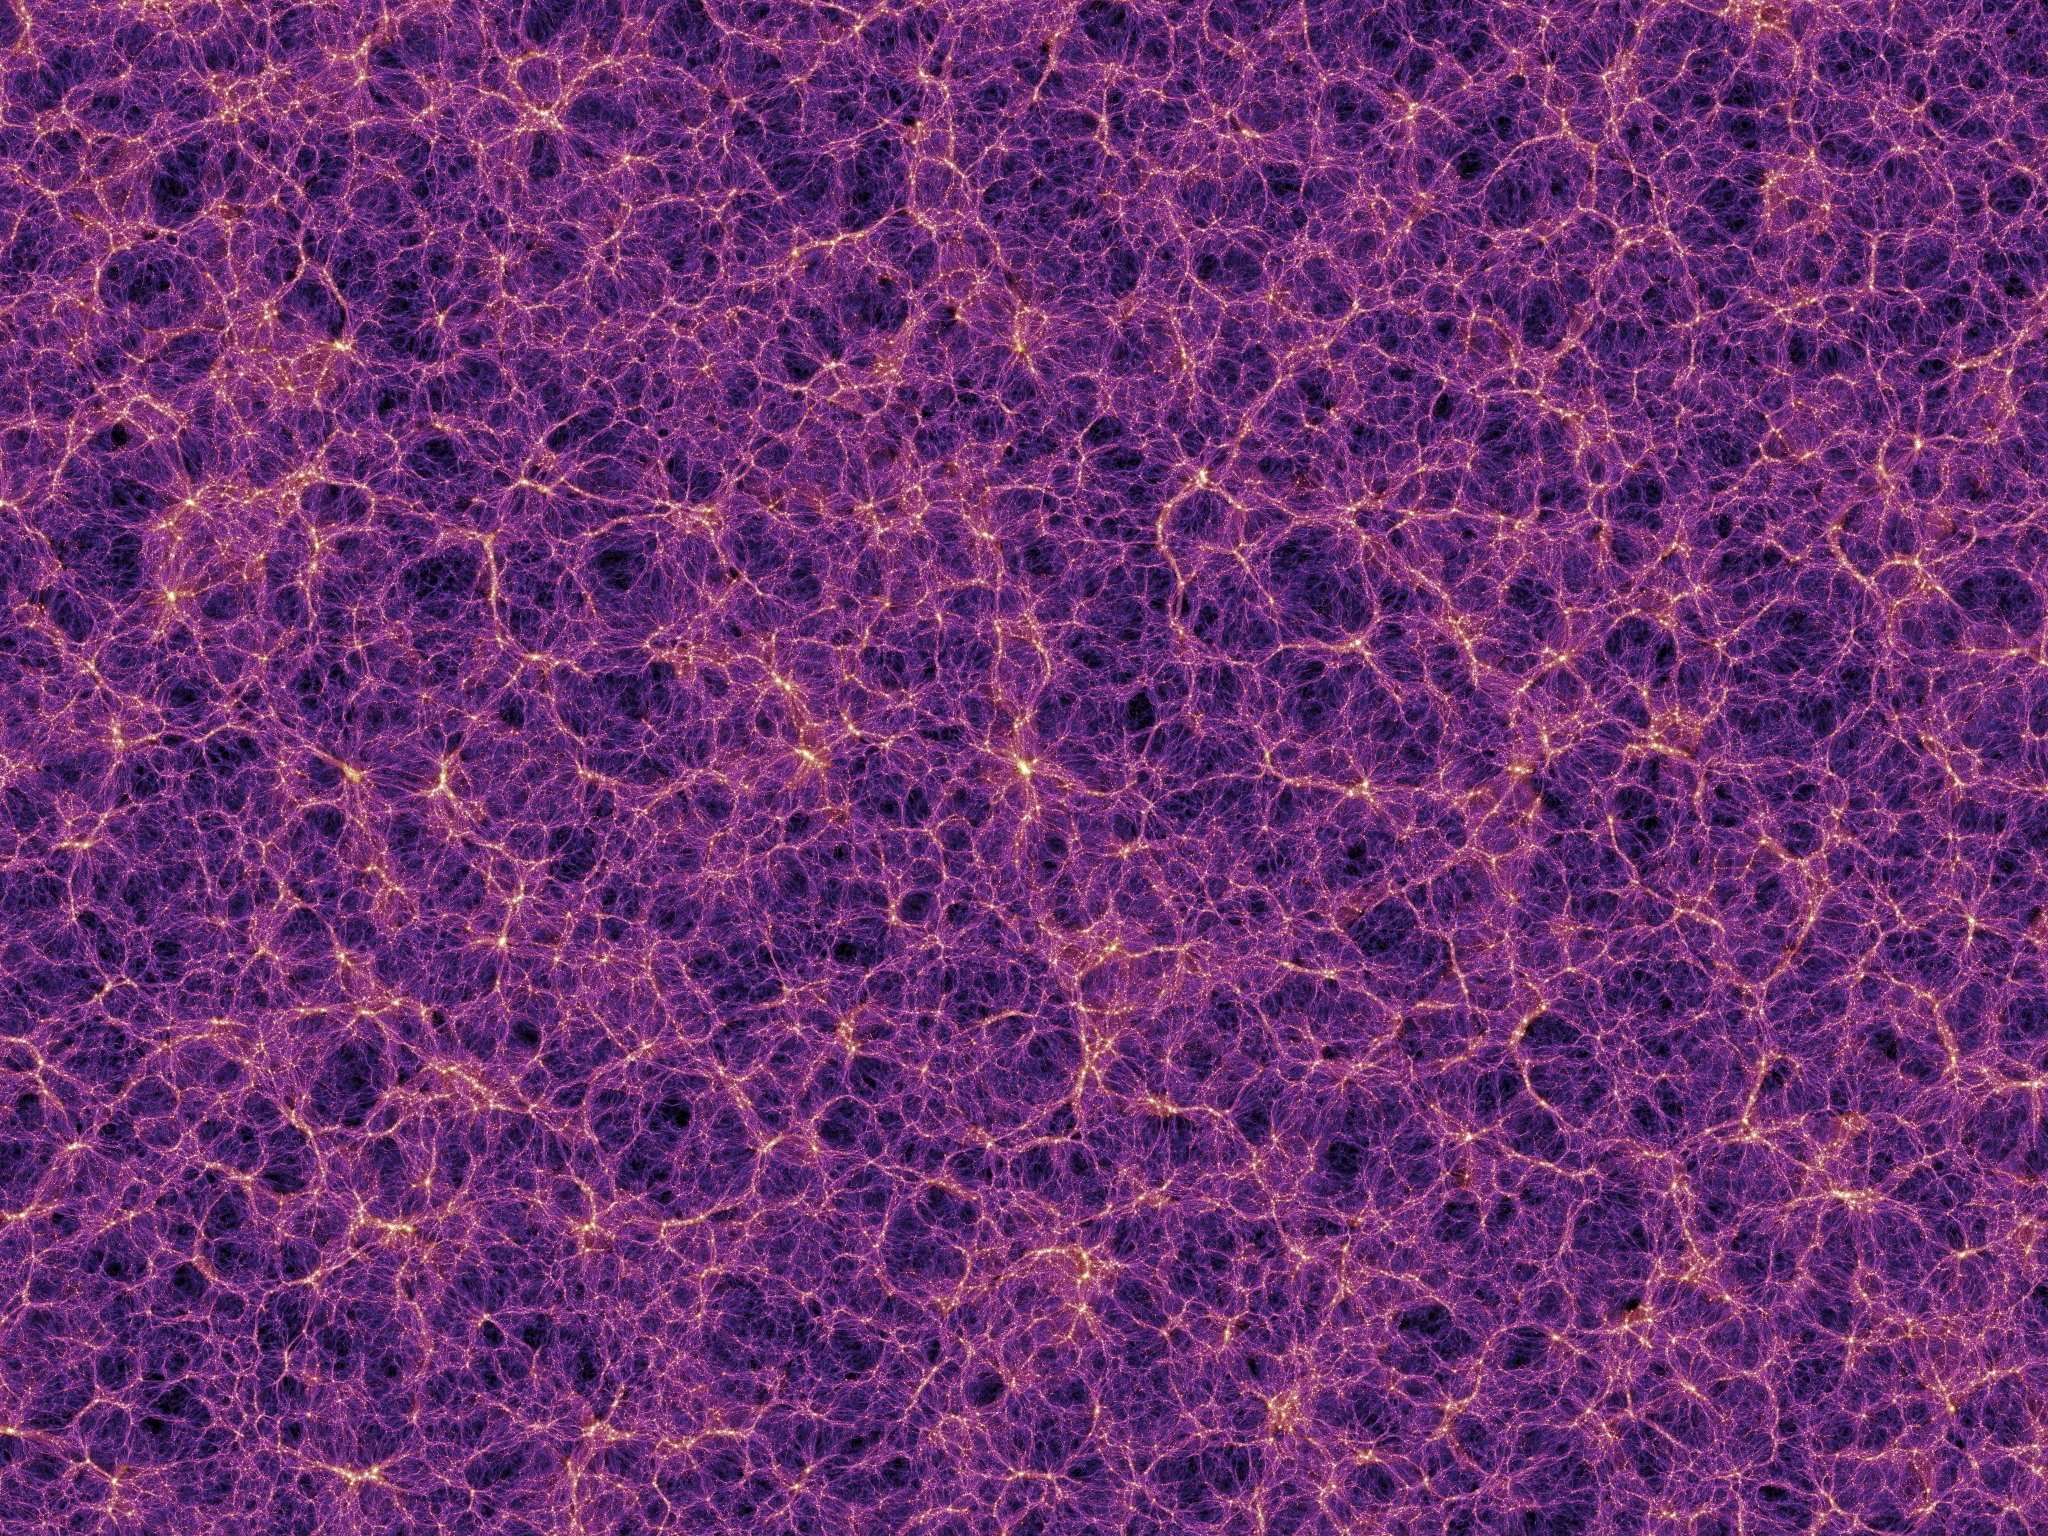
\includegraphics[height=3.4cm]{figures/millennium_many_body}\\
       {\footnotesize Source: Millennium Simulation}\\
       \vspace{0.2cm}
       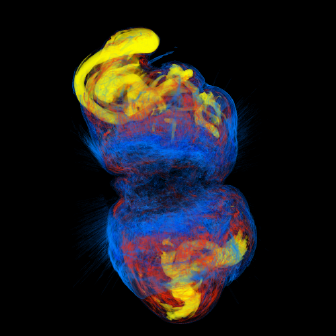
\includegraphics[height=3.4cm]{figures/Beta_volren_0123_small}\\
       {\footnotesize Source: M\"{o}sta et al.}
       \vspace{0.1cm}
     \end{center}
     \column{6cm}
     \begin{center}
       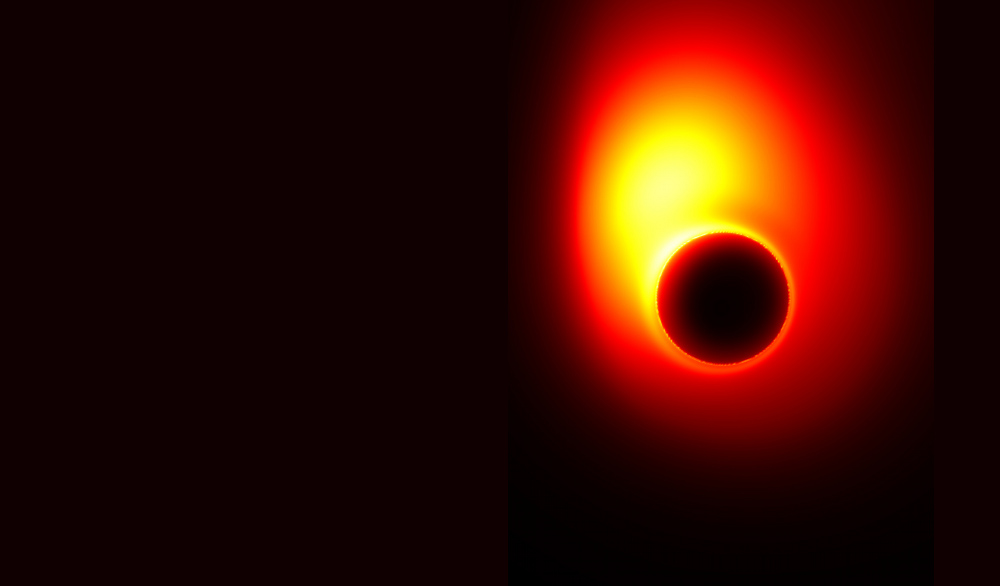
\includegraphics[height=3.4cm]{figures/black-hole-shadow}\\
       {\footnotesize Source: Avery Broderick}\\
       \vspace{0.2cm}
       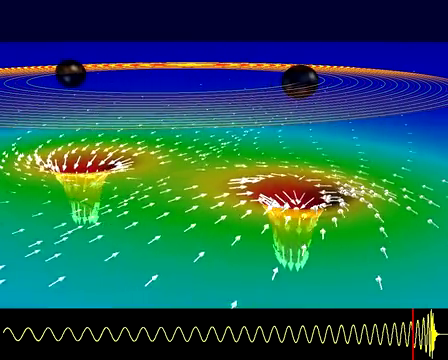
\includegraphics[height=3.4cm]{figures/bbh_sxs}\\
       {\footnotesize Source: The SXS Collaboration}
       \vspace{0.1cm}
     \end{center}
  \end{columns}
\end{frame}

\section{Structure of a Star}
\label{sec:star}

\begin{frame}
  \frametitle{Math is our X-Ray Vision}
  \begin{center}
    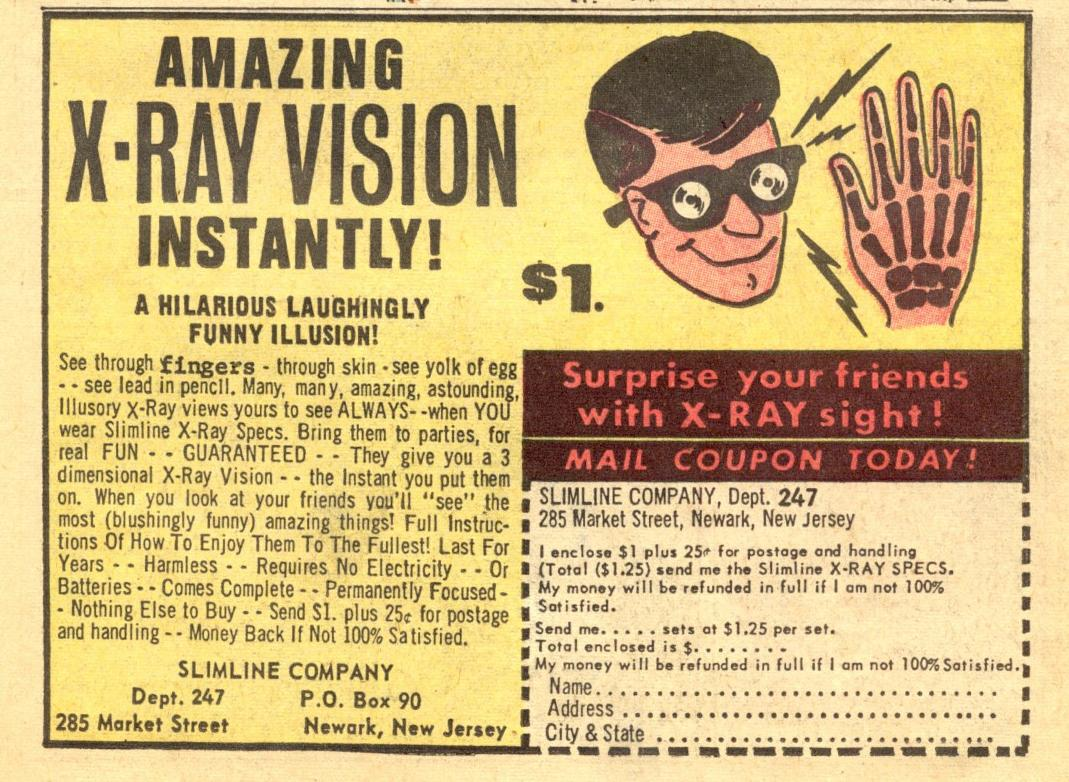
\includegraphics[height=8cm]{figures/xrayspex}\\
    {\footnotesize Source: Comic Book Resources}
  \end{center}
\end{frame}

\begin{frame}
  \frametitle{Seeing Inside a Star}
  \setlength{\unitlength}{1cm}
  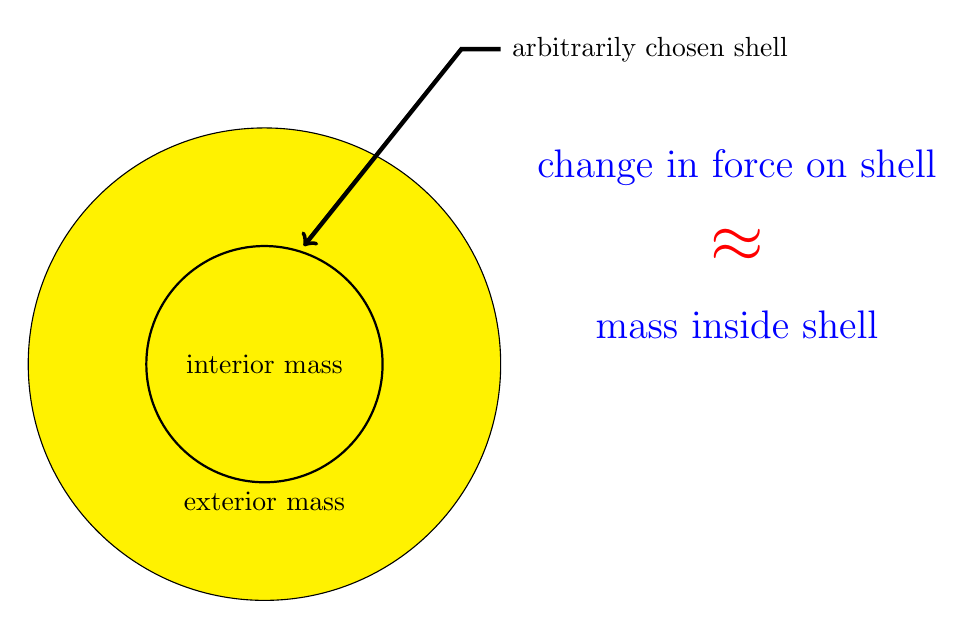
\begin{tikzpicture}
    \coordinate (scenter) at (3.5cm,4cm);
    \filldraw[fill=yellow,draw=black] (scenter) circle (3cm);
    \draw[thick,black] (scenter) circle (1.5cm);
    \draw (scenter) node {interior mass};
    \draw (3.5cm,2.5cm) node[below] {exterior mass};
    \draw[ultra thick,black,<-] (4,5.5) 
    -- (6,8) -- (6.5,8) node[right] {arbitrarily chosen shell};
    \draw (9.5,6.5) node {\Large \color{blue} change in force on shell};
    \draw (9.5,5.5) node {\Huge \color{red} $\approx$};
    \draw (9.5,4.5) node {\Large \color{blue} mass  inside shell};
  \end{tikzpicture}
\end{frame}

\begin{frame}
  \frametitle{Mass, Radius}
  \begin{center}
    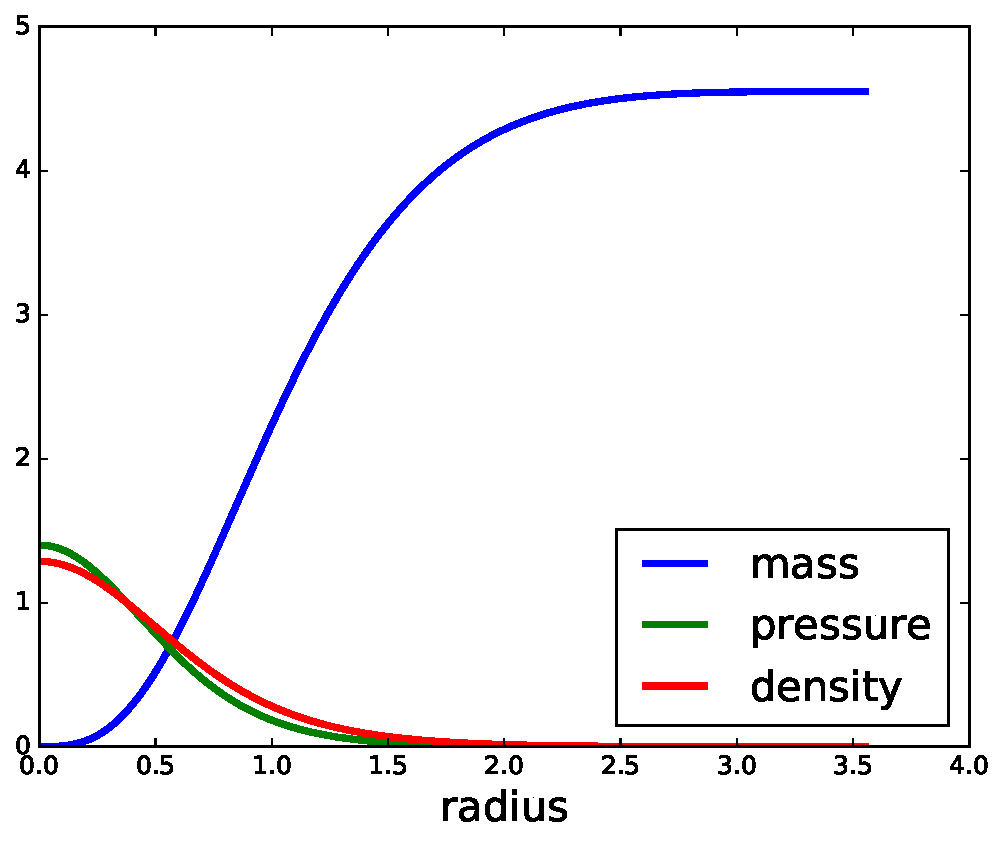
\includegraphics[height=8cm]{figures/star_profile}
  \end{center}
\end{frame}

\begin{frame}
  \frametitle{Mass, Radius}
  \setlength{\unitlength}{1cm}
  \begin{picture}(12,8)
    \put(0,0){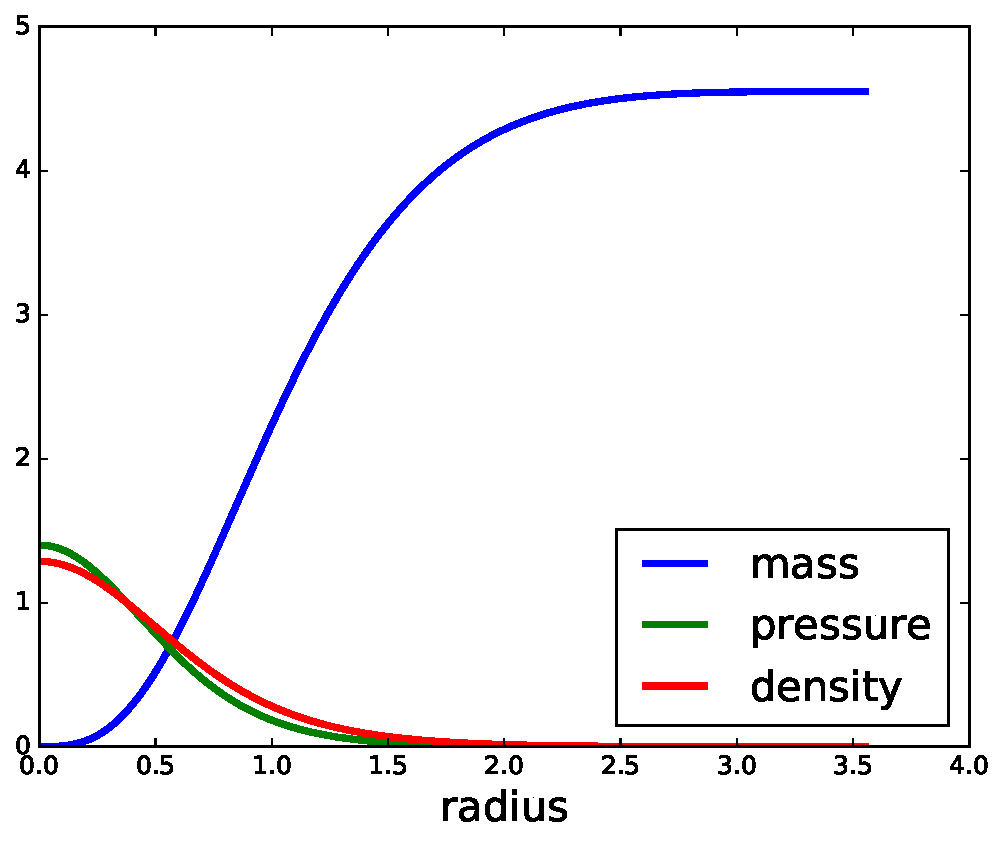
\includegraphics[width=4cm]{figures/star_profile}}
    \put(2,2){\fcolorbox{black}{white}{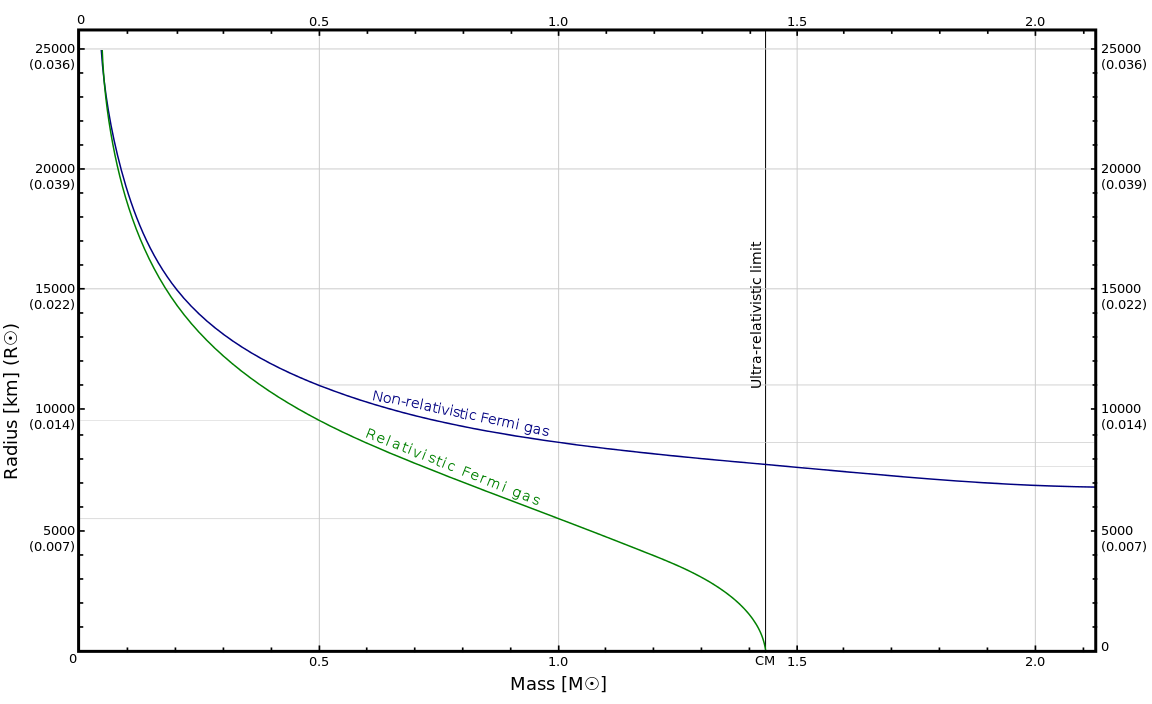
\includegraphics[width=10cm]{figures/mass_vs_radius}}}
    \put(5,1.5){\footnotesize Source: Wikimedia Commons}
  \end{picture}
\end{frame}

\begin{frame}
  \frametitle{Code}
  \begin{itemize}
  \item These slides:\\ 
    {\small\url{https://github.com/Yurlungur/computational-physics-demos}}
  \item Monte Carlo for $\pi$:\\
    {\small\url{https://bitbucket.org/Yurlungur/pi_monte_carlo}}
  \item Newton's Laws:\\ 
    {\small\url{https://github.com/Yurlungur/forward-euler-demo}}
  \item Stellar Structure:\\ 
    {\small \url{https://github.com/Yurlungur/stellar-structure}}
  \end{itemize}
\end{frame}

\end{document}